% !TEX root=../pldi2019.tex



\section{Language}



\subsection{Base language}

Let us start by defining our host language.
It is a simple $\lambda$-calculus.
Next to abstraction, application and variables,
it contains constants for booleans, integers and strings
and some basic operations on them.
We will embed our task language \emph{into} this basic language.
This means we can use all the power of the host language,
such as arithmetic operations and (higher order) functions,
in our task language.
Because all the constructs in our host language are standard,
we will not give typing rules and semantic rules here.
For this we refer to standard work like \textcite{books/Pierce02TAPL} and \textcite{books/Harper16PFPL}.

Expressions are typed abstractions, applications, variables or constants.
Constants can be booleans, integers or strings.
The $\star$ represents a general notion of operators.
With $\If{}{}{}$ one can do basic branching.
The syntactic category of pretasks will be defined in the upcoming sections.
Pretasks $p$ are tasks \emph{in making},
just as expressions are values in making.
A \emph{task} will be introduced in \autoref{sec:evaluation}.

We will use double quotation marks ($\str{}$) to denote strings.
Integers are denoted by their decimal representation,
and booleans are written $\True$ and $\False$.
In the remaining of this report,
we will freely make use of the logic operators $\Not$, $\land$, and $\lor$,
arithmetic operators $+$, $-$, $\times$,
and the string append operator $\pp$.
Also, we will use the standard comparison operations $<$, $\le$, $\equiv$, $\not\equiv$, $\ge$, and $>$
as builtins.
Only when referring to operators in general we will use $\star$.

\todo{Make grammars more compact?}

\begin{figure}
  \usemacro{G-Language}
  \caption{Language grammar} \label{fig:language-grammar}
\end{figure}

\begin{figure}
  \usemacro{G-Pretasks}
  \caption{Task grammar} \label{fig:task-grammar}
\end{figure}


\subsection{Typing}

Typing of our expressions $e$ is as to be expected,
and won't be given in this document.
There is one big difference with respect to standard work.
This is the addition of a type for tasks $\Task \tau$.
Typing rules are of the form $\Gamma \infers e : \tau$,
which we read as \enquote{in environment $\Gamma$, expression $e$ has type $\tau$}.

\begin{figure}
  \usemacro{G-Types}
  \caption{Type grammar} \label{fig:type-grammar}
\end{figure}

\begin{figure}
  \small
  \begin{mathpar}
    \boxed{\RelationT} \\
    \userule{T-Edit} \quad
    \userule{T-Fill} \quad
    \userule{T-Update} \\
    \userule{T-Then} \\
    \userule{T-Next} \\
    \userule{T-And} \\
    \userule{T-Or} \\
    \userule{T-Xor}\\
    \userule{T-Appoint} \quad
    \userule{T-Fail} \\
  \end{mathpar}
  \caption{Typing rules} \label{fig:typing-rules}
\end{figure}



\subsection{Editors}

In the introduction we claimed to create a language to model \emph{interactive} workflows.
By interaction we mean \emph{communication with people using the developed system}.
These \emph{end users} should be able to enter information into the system,
change it, clear it, reenter it, etc.
To do this, we introduce the concept of an \emph{editor}.

Editors may or may not contain a current value.
When an editor has a value, it can be \emph{changed} or it can be \emph{emptied}.
When it is empty, a value can be \emph{filled}.
This is depicted as a state diagram in \autoref{fig:editor-state} below.

\begin{figure}
  \centering
  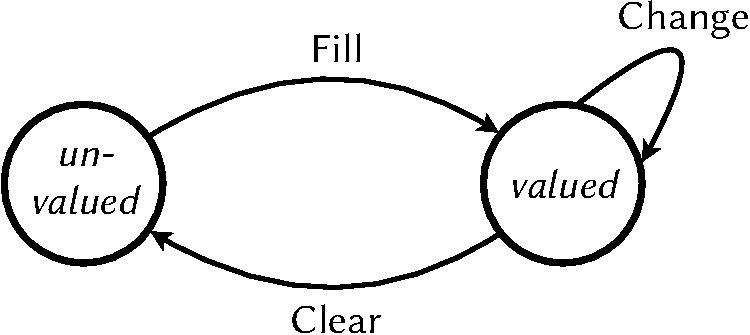
\includegraphics[width=0.6\columnwidth]{figures/drawings-crop.pdf}
  \caption{Possible states of an editor and its transitions.}
  \label{fig:editor-state}
\end{figure}

One can consider editors as an abstraction over widgets in a \GUI,
form fields on a webpage,
or even sensors plugged into the system.
Take for example an entry for text.
Users can enter a string, change it, remove it, enter another string, and so on.
With editors we try to capture this \emph{constantly changing} nature of user input.
Also, because editors are \emph{typed},
they are only allowed to contain information of the right format.

How exactly information is entered is not of great importance.
This could be an input field for a string,
a switch for a boolean,
a spin box for an angle,
or even a map with a pin for a location.
\Autoref{fig:editor-examples} depicts these examples.
In it's most banal form,
an editor is a line of text entered at a terminal and parsed to match a string, boolean, angle or location value.

Valued editors contain an expression $e$.
Therefore they inherit the type of $e$,
but embedded in the container type $\Task$.
For now, we only accept expressions of a basic type $\beta$ as a value of an editor.
This is expressed by the following typing rule for valued editors.
\refrule{T-Edit}

Unvalued editors do not have a value,
and therefore do not wrap an expression.
Because we strive to a fully typed system,
we have two options to type unvalued editors:
\begin{enumerate*}
  \item let the unvalued editor have a polymorphic type;
  \item annotate unvalued editors with a type and use that. \label{itm:annotate}
\end{enumerate*}

The first option sounds appealing.
However, consider the following use case.
We start with an editor containing the value two: $\Edit 2$.
The user can change this value, as long as it is an integer,
for example to five: $\Edit 5$.
Clearing the value results in an unvalued editor: $\Enter$.
Now, are we allowed to enter a value of some other type?
That is, can we now enter a string?
This would change the type of the editor!

Therefore,
we need to keep track of the type of values that can be entered into an unvalued editor
and we choose option (\ref{itm:annotate}).
The typing rule becomes:
\refrule{T-Fill}

Some examples of editors expressible in our language:
\begin{itemize}
  \item $\Edit 2$ is a valued editor which contains the integer value $2$.
  \item $\Enter \String$ is an unvalued editor,
    waiting for users to enter some string.
  \item $\Edit ((\lambda x . x)\ 5)$ is a valued editor which,
    after evaluation, will contain the value $5$.
    (We will discuss evaluation of editors in the next section.)
\end{itemize}

At the core,
an editor is a container holding a value
or holding nothing.
For this purpose, we extend our task language with two constructs:
a valued editor $\Edit e$ and an unvalued editor $\Enter \beta$.



\subsection{Steps}

In the previous section we have set up our interaction model of inputs and actions,
we defined our interactive component, the editor,
and introduced the infinitely failing task.
Now that we have the core part of an interactive workflow,
we can continue with ways to compose multiple tasks.
Combining tasks can be done in two ways:
\begin{enumerate*}
  \item sequential or
  \item parallel.
\end{enumerate*}
For parallel composition we distinguish two kinds:
\begin{enumerate*}[(a)]
  \item pairing two tasks (\emph{and}-parallel); and
  \item choosing between two tasks (\emph{or}-parallel).
\end{enumerate*}
In this section we start with sequential composition.
The next two sections are about pairing and choosing.

One might think that the best way to sequence tasks is by just following one task with another:
do this, then do that, then that, etc.
However, we like the continuation to depend on the value produced by the preceding task.
\todo{Elaborate more about the reasons for this.}
This is done by a \emph{step}.
We define a step from one task to another as
\begin{quote}
  a calculation which returns the next task to proceed with.
\end{quote}

To accomplish this,
we take continuations to be \emph{functions}.
These are just normal functions from our host language which,
when evaluated, result in something of type $\Task$.
Therefore,
we extend our pretasks $p$ with a sequence construct $\Then$.

The accompanied typing rule looks like
\refrule{T-Then}
Note that typing ensures us that the left hand side $e_1$ will be a task delivering a value of type $\tau_1$.
The right hand side $e_2$ then, will use this value of type $\tau_1$,
and calculate a \emph{new} task holding a value of (possibly another) type $\tau_2$.

Evaluation of a sequence is done by only evaluating the left hand side, $e_1$,
as this expression is be something of type $\Task \tau_1$.
As the right hand side, $e_2$, is a function,
it does not matter if we evaluate $e_2$ right away or store it lazily.
\refrule{E-Then}
Consequentially, we extend our tasks $t$ with an evaluated sequence construct.



\subsection{Composition}

\paragraph{Parallel}

\paragraph{Choice}

\paragraph{Appointing}


\subsection{State}
